\section{Analysis}
\label{sec:analysis}

\subsection{Third-party systems}
\label{sec:external}

\begin{table*}[t]
\caption{Third-party systems on SWE-bench Lite, each next to our trained ranker on exactly the issues it ran on. Recall cells are theirs / ours, in percent. The difference is paired over the same issues, with a 95\% bootstrap interval. Seconds per file include model scoring on our laptop GPU.}
\label{tab:external}
\centering
\scriptsize
\setlength{\tabcolsep}{3pt}
\resizebox{\textwidth}{!}{\T{lite_external}}
\end{table*}

Table~\ref{tab:external} compares the two released systems with our ranker. Both ran from the authors' code, with changes needed only to run them on our machine. SWE-Pruner ran on all of Lite. In its released form it keeps the lines whose score is above a threshold, which gives no control over the output size, so we take its line scores exactly as the authors compute them and keep the best lines until the budget is full. LongCodeZip's paper uses a 7B scoring model. On our 8\,GB GPU we used Qwen2.5-Coder-1.5B-Instruct and a fixed random sample of 100 Lite issues with gold files only. Its full two-stage mode takes 30 to 60 seconds per file and was stopped by a three-hour cap after 42 of those issues. These rows show what the systems do under our hardware, not the best they can do. The details are in \texttt{docs/baselines.md}.

On gold-function recall our ranker is far ahead of both. Against SWE-Pruner at the 25\% budget the paired difference is \dif{lite:oracle_imports:ast_trained:swe_pruner:r0.25} points with imports and \dif{lite:oracle:ast_trained:swe_pruner:r0.25} with gold files only. On gold-line recall, the metric that suits a line pruner, the picture changes. SWE-Pruner is level with our ranker when imports are included (\res{lite:oracle_imports:swe_pruner:r0.25:gold_line_recall}\% against \res{lite:oracle_imports:ast_trained:r0.25:gold_line_recall}\% at 25\%) and ahead with gold files only at the 10\% budget (\res{lite:oracle:swe_pruner:r0.10:gold_line_recall}\% against \res{lite:oracle:ast_trained:r0.10:gold_line_recall}\%). So a trained line scorer finds the edited lines about as well as our ranker. What it does not do is keep the function around them intact. Its pruned views parse as Python in \res{lite:oracle_imports:swe_pruner:r0.25:parse_rate}\% of cases, and it needs several seconds per file where our ranker needs a fraction of a second.

LongCodeZip's coarse stage ranks whole functions by how much each one lowers the perplexity of the query, which makes it the closest relative of our method. On its 95 issues it keeps \res{lite:oracle:longcodezip_rank:r0.25:gold_fn_recall}\% of gold functions at 25\%, about what BM25 keeps on the same issues. Our ranker keeps \dif{lite:oracle:ast_trained:longcodezip_rank:r0.25} points more (\dif{lite:oracle:ast_trained:longcodezip_rank:r0.25:lo} to \dif{lite:oracle:ast_trained:longcodezip_rank:r0.25:hi}). The full mode keeps fewer, \res{lite:oracle:longcodezip:r0.25:gold_fn_recall}\% on 40 issues. Part of the reason is that its budget is a soft target: when allowed 25\% of the tokens it uses \res{lite:oracle:longcodezip:r0.25:compression}\%.

\subsection{Scaling and cost}

\begin{figure}[t]
\centering
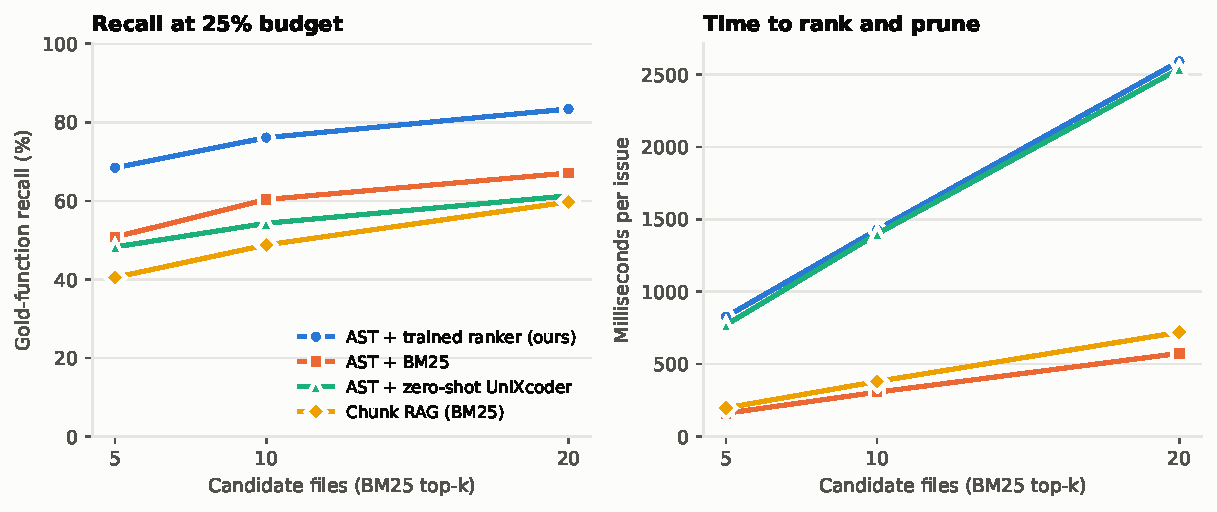
\includegraphics[width=\columnwidth]{lite_scaling}
\caption{Gold-function recall at a 25\% budget as the number of BM25-retrieved candidate files grows, SWE-bench Lite.}
\label{fig:scaling}
\end{figure}

With retrieved files, recall rises with the number of candidate files for every method (Fig.~\ref{fig:scaling}), because more files means the gold file is retrieved more often and a 25\% budget holds more tokens. The order of the methods does not change. With 20 files the trained ranker keeps \stat{scaling:lite:ast_trained:20:recall}\% of gold functions and BM25 on the same nodes \stat{scaling:lite:ast_bm25:20:recall}\%.

The ranker is cheap to run. It has \stat{train:main:params_m}M parameters and needs no language model at inference time. Timed over \stat{scaling:lite:issues} issues with cold caches on the laptop GPU, an issue with 20 candidate files takes \stat{scaling:lite:ast_trained:20:ms}\,ms, of which \stat{scaling:lite:ast_trained:20:score_ms}\,ms is scoring and \stat{scaling:lite:ast_trained:20:select_ms}\,ms is selection. That is \stat{scaling:lite:ast_trained:20:ms_file}\,ms per file, against \stat{scaling:lite:ast_bm25:20:ms_file}\,ms for BM25.

\subsection{Where the ranker fails}

We collected every gold function that the trained ranker and BM25 lost on Lite at the 25\% budget, with gold files and their imports, and sorted them by simple rules (\texttt{docs/error\_analysis.md}). The trained ranker loses \stat{errors:ast_trained:total} of \stat{lite:gold_functions_total} gold functions and BM25 loses \stat{errors:ast_bm25:total}. For both, most losses are functions that the issue never names and that other code outranked: \stat{errors:ast_trained:3} for our ranker and \stat{errors:ast_bm25:3} for BM25. Such issues describe a symptom, such as an error, a wrong result or a server that does not restart, and the fix sits in code with different names. This is where training helps most. BM25 also often reaches the gold function only after its body no longer fits, and shows a signature (\stat{errors:ast_bm25:2} cases, against \stat{errors:ast_trained:2} for our ranker). Functions that are larger than half the budget account for \stat{errors:ast_trained:1} losses for each method.

Three cases show the patterns. In \texttt{django-15388} the development server stops restarting once a setting changes. The fix is in \texttt{template\_changed} in the template autoreloader, a function the issue never names. BM25 ranks it 37th of 79 nodes and drops it, and the trained ranker keeps it. In \texttt{sympy-13146} a user finds that \texttt{-0.5*x**2.5 + 0.5*x**2.5} does not simplify to zero after \texttt{evalf}. The fix is in \texttt{AssocOp.\_eval\_evalf}, deep in SymPy's core, and the issue names neither the method, its class nor its module. Our ranker places it 184th of 576 nodes and loses it. In \texttt{django-15851} the ranker puts the right function first, but at 359 tokens it is larger than the whole 166-token budget, so it is shown as a signature. The agent then knows which function to open and can ask again with a larger budget, but our metric counts the case as lost.
